%%%%%%%%%%%%%%%%%%%%%%%%%%%%%%%%%%%%%%%%%%%%%%%%%%%%%%%%%%%%%%%%%%%%%%%%%%%%%%%%%%%%%%%%%%%%%%%%%%%%%%
% Plantilla básica de Latex en Español.
%
% Autor: Andrés Herrera Poyatos (https://github.com/andreshp) 
%
% Es una plantilla básica para redactar documentos. Utiliza el paquete fancyhdr para darle un
% estilo moderno pero serio.
%
% La plantilla se encuentra adaptada al español.
%
%%%%%%%%%%%%%%%%%%%%%%%%%%%%%%%%%%%%%%%%%%%%%%%%%%%%%%%%%%%%%%%%%%%%%%%%%%%%%%%%%%%%%%%%%%%%%%%%%%%%%%

%-----------------------------------------------------------------------------------------------------
%	INCLUSIÓN DE PAQUETES BÁSICOS
%-----------------------------------------------------------------------------------------------------

\documentclass{article}


%-----------------------------------------------------------------------------------------------------
%	SELECCIÓN DEL LENGUAJE
%-----------------------------------------------------------------------------------------------------

% Paquetes para adaptar Látex al Español:
\usepackage[spanish,es-noquoting, es-tabla, es-lcroman]{babel} % Cambia 
\usepackage[utf8]{inputenc}                                    % Permite los acentos.
\selectlanguage{spanish}                                       % Selecciono como lenguaje el Español.

%-----------------------------------------------------------------------------------------------------
%	SELECCIÓN DE LA FUENTE
%-----------------------------------------------------------------------------------------------------

% Fuente utilizada.
\usepackage{courier}                    % Fuente Courier.
\usepackage{microtype}                  % Mejora la letra final de cara al lector.

%-----------------------------------------------------------------------------------------------------
%	ESTILO DE PÁGINA
%-----------------------------------------------------------------------------------------------------

% Paquetes para el diseño de página:
\usepackage{fancyhdr}               % Utilizado para hacer títulos propios.
\usepackage{lastpage}               % Referencia a la última página. Utilizado para el pie de página.
\usepackage{extramarks}             % Marcas extras. Utilizado en pie de página y cabecera.
\usepackage[parfill]{parskip}       % Crea una nueva línea entre párrafos.
\usepackage{geometry}               % Asigna la "geometría" de las páginas.

% Se elige el estilo fancy y márgenes de 3 centímetros.
\pagestyle{fancy}
\geometry{left=3cm,right=3cm,top=3cm,bottom=3cm,headheight=1cm,headsep=0.5cm} % Márgenes y cabecera.
% Se limpia la cabecera y el pie de página para poder rehacerlos luego.
\fancyhf{}

% Espacios en el documento:
\linespread{1.1}                        % Espacio entre líneas.
\setlength\parindent{0pt}               % Selecciona la indentación para cada inicio de párrafo.

% Cabecera del documento. Se ajusta la línea de la cabecera.
\renewcommand\headrule{
	\begin{minipage}{1\textwidth}
	    \hrule width \hsize 
	\end{minipage}
}

% Texto de la cabecera:
\lhead{\subject}                          % Parte izquierda.
\chead{}                                    % Centro.
\rhead{\doctitle \ - \docsubtitle}              % Parte derecha.

% Pie de página del documento. Se ajusta la línea del pie de página.
\renewcommand\footrule{                                 
\begin{minipage}{1\textwidth}
    \hrule width \hsize   
\end{minipage}\par
}

\lfoot{}                                                 % Parte izquierda.
\cfoot{}                                                 % Centro.
\rfoot{Página\ \thepage\ de\ \protect\pageref{LastPage}} % Parte derecha.


%----------------------------------------------------------------------------------------
%   MATEMÁTICAS
%----------------------------------------------------------------------------------------

% Paquetes para matemáticas:                     
\usepackage{amsmath, amsthm, amssymb, amsfonts, amscd} % Teoremas, fuentes y símbolos.
     
 % Nuevo estilo para definiciones
 \newtheoremstyle{definition-style} % Nombre del estilo
 {5pt}                % Espacio por encima
 {0pt}                % Espacio por debajo
 {}                   % Fuente del cuerpo
 {}                   % Identación: vacío= sin identación, \parindent = identación del parráfo
 {\bf}                % Fuente para la cabecera
 {.}                  % Puntuación tras la cabecera
 {.5em}               % Espacio tras la cabecera: { } = espacio usal entre palabras, \newline = nueva línea
 {}                   % Especificación de la cabecera (si se deja vaía implica 'normal')
 
 % Nuevo estilo para teoremas
 \newtheoremstyle{theorem-style} % Nombre del estilo
 {5pt}                % Espacio por encima
 {0pt}                % Espacio por debajo
 {\itshape}           % Fuente del cuerpo
 {}                   % Identación: vacío= sin identación, \parindent = identación del parráfo
 {\bf}                % Fuente para la cabecera
 {.}                  % Puntuación tras la cabecera
 {.5em}               % Espacio tras la cabecera: { } = espacio usal entre palabras, \newline = nueva línea
 {}                   % Especificación de la cabecera (si se deja vaía implica 'normal')
 
 % Nuevo estilo para ejemplos y ejercicios
 \newtheoremstyle{example-style} % Nombre del estilo
 {5pt}                % Espacio por encima
 {0pt}                % Espacio por debajo
 {}                   % Fuente del cuerpo
 {}                   % Identación: vacío= sin identación, \parindent = identación del parráfo
 {\scshape}                % Fuente para la cabecera
 {:}                  % Puntuación tras la cabecera
 {.5em}               % Espacio tras la cabecera: { } = espacio usal entre palabras, \newline = nueva línea
 {}                   % Especificación de la cabecera (si se deja vaía implica 'normal')
 
 % Teoremas:
 \theoremstyle{theorem-style}  % Otras posibilidades: plain (por defecto), definition, remark
 \newtheorem{theorem}{Teorema}[section]  % [section] indica que el contador se reinicia cada sección
 \newtheorem{corollary}[theorem]{Corolario} % [theorem] indica que comparte el contador con theorem
 \newtheorem{lemma}[theorem]{Lema}
 \newtheorem{proposition}[theorem]{Proposición}
 
 % Definiciones, notas, conjeturas
 \theoremstyle{definition}
 \newtheorem{definition}{Definición}[section]
 \newtheorem{conjecture}{Conjetura}[section]
 \newtheorem*{note}{Nota} % * indica que no tiene contador
 
 % Ejemplos, ejercicios
 \theoremstyle{example-style}
 \newtheorem{example}{Ejemplo}[section]
 \newtheorem{exercise}{Ejercicio}[section]

%-----------------------------------------------------------------------------------------------------
%	BIBLIOGRAFÍA
%-----------------------------------------------------------------------------------------------------

\usepackage[backend=bibtex, style=numeric]{biblatex}
\usepackage{csquotes}

\addbibresource{references.bib}

%-----------------------------------------------------------------------------------------------------
%	PORTADA
%-----------------------------------------------------------------------------------------------------

% Elija uno de los siguientes formatos.
% No olvide incluir los archivos .sty asociados en el directorio del documento.
\usepackage{title1}
%\usepackage{title2}
%\usepackage{title3}

%-----------------------------------------------------------------------------------------------------
%	TÍTULO, AUTOR Y OTROS DATOS DEL DOCUMENTO
%-----------------------------------------------------------------------------------------------------

% Título del documento.
\newcommand{\doctitle}{Ecuaciones diferenciales ordinarias}
% Subtítulo.
\newcommand{\docsubtitle}{Método del trapecio}
% Fecha.
\newcommand{\docdate}{1 \ de \ Enero \ de \ 2015}
% Asignatura.
\newcommand{\subject}{Métodos Numéricos II}
% Autor.
\newcommand{\docauthor}{Andrés Herrera Poyatos \\ Javier Poyatos Amador \\ Rodrigo Raya Castellano}
\newcommand{\docaddress}{Universidad de Granada}
\newcommand{\docemail}{}

%-----------------------------------------------------------------------------------------------------
%	RESUMEN
%-------------------------------					----------------------------------------------------------------------

% Resumen del documento. Va en la portada.
% Puedes también dejarlo vacío, en cuyo caso no aparece en la portada.
%\newcommand{\docabstract}{}
\newcommand{\docabstract}{En este texto puedes incluir un resumen del documento. Este informa al lector sobre el contenido del texto, indicando el objetivo del mismo y qué se puede aprender de él.}

\begin{document}

\maketitle

%-----------------------------------------------------------------------------------------------------
%	ÍNDICE
%-----------------------------------------------------------------------------------------------------

% Profundidad del Índice:
%\setcounter{tocdepth}{1}

\newpage
\tableofcontents
\newpage

%-----------------------------------------------------------------------------------------------------
%	SECCIÓN 1: MOTIVACIÓN
%-----------------------------------------------------------------------------------------------------

\section{Motivación: resolución de ecuaciones diferenciales ordinarias}
\begin{definition} Dada una función $f:\Omega \subseteq \mathbb R^2  \to \mathbb{R}$ un problema de valores iniciales de primer orden consiste en encontrar aquellas funciones $y$ tal que $y'(t) = f(t,y(t))$ y se verifique la condición inicial $y(a) = y_0$.  
\end{definition}

	Uno de los objetivos de la teoría del Análisis numérico en el campo de las ecuaciones diferenciales ordinarias es resolver de forma aproximada computacionalmente problemas de valores iniciales. De forma simplificada estos problemas pueden expresarse así:

\begin{center}
$\begin{cases}
y'(t) = f(t,y(t)) \\
y(a) = y_0 \\
t \in [a,b] \\
\end{cases}$
\end{center}

La primera idea intuitiva para resolver este problema consiste en interpretar la primera ecuación como un campo vectorial aprovechando la definición de derivada como aproximación lineal de la función en un punto:

\begin{figure}[h]
\centering
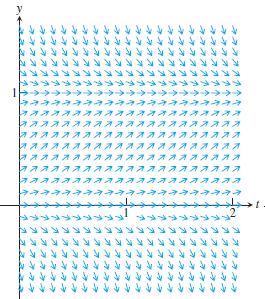
\includegraphics[width=4cm]{./Images/interpret-pvi.png}
\caption{Representación del campo vectorial asociado a la ecuación logística.} 
\label{fig:interpret-pvi}
\end{figure}

De este modo nace el método de Euler cuya expresión resumida es la siguiente:

\begin{center}
$\begin{cases}
w_0=y_0 \\
w_{i+1} = w_i + h f(t_i,w_i)
\end{cases}$
\end{center}

Veremos a continuación un ejemplo de por qué no es suficiente con el método de Euler. Previamente, necesitamos conocer algunos resultados básicos sobre la existencia, unicidad y condicionamiento de las soluciones:

\begin{theorem}
\begin{itemize}
\item Si f es Lipschitz en $[a,b]\times[\alpha,\beta]$ y $\alpha < y_a < \beta$ entonces existe $c \in [a,b]$ tal que el problema de valores iniciales:
\begin{center}
$\begin{cases}
y'(t) = f(t,y(t)) \\
y(a) = y_0 \\
t \in [a,c] \\
\end{cases}$
\end{center}
tiene exactamente una solución. 
\item Si f es Lipschitz en $[a,b]\times]-\infty,\infty[$ entonces existe exactamente una solución en $[a,b]$
\item (Condicionamiento) Si f es Lipschitz en $[a,b]\times[\alpha,\beta]$ e Y(t), Z(t) son soluciones en $[a,b]\times[\alpha,\beta]$ del problema de valores iniciales con ecuación $y'(t) = f(t,y(t))$ y condiciones iniciales $Y(a)$ y $Z(a)$ entonces $|Y(t)-Z(t)| \leq e^{L(t-a)}|Y(a)-Z(a)|$ donde L es la constante de Lipschitz de f.
\end{itemize}
\end{theorem}

Necesitamos también medir de algún modo cómo de bueno es el procedimiento utilizado para aproximar la solución del problema para ello se introduce la siguiente:

\begin{definition} Sean $w_i$ los valores estimados en los puntos $t_i$ por cierto método de aproximación de las soluciones del problema de valores iniciales:
\begin{center}
$\begin{cases}
y'(t) = f(t,y(t)) \\
y(a) = y_a \\
t \in [a,b] \\
\end{cases}$
\end{center}
e $y_i$ los valores exactos de la solución en los puntos $t_i$. Sea también $z(t_i)$ el valor de la solución exacta al problema de valores iniciales:
\begin{center}
$\begin{cases}
y'(t) = f(t,y(t)) \\
y(t_i) = w_i \\
t \in [t_i,t_{i+1}] \\
\end{cases}$
\end{center}
Definimos:
\begin{itemize}
\item Error global de truncatura o error acumulado en el nodo i-ésimo: $g_i=|w_i-y_i|$
\item Error local de truncatura o error en un paso: $e_{i+1} = |w_i-z(t_{i+1})|$
\end{itemize} 
\end{definition}

El error global cometido en cualquier paso puede verse entonces como la suma del error local y el error global acumulado o amplificado. Para el método de Euler los errores global y local pueden visualizarse fácilmente:

\begin{figure}[h]
\centering
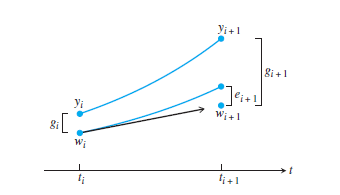
\includegraphics[width=10cm]{./Images/error-euler.png}
\caption{Error local y global cometido por el método de Euler} 
\label{fig:error-euler}
\end{figure}

La relación entre errores locales y errores globales viene dada por el siguiente:

\begin{theorem}
Si f es Lipschitz con constante L, $y_i$ son los valores de la solución a un problema de valores iniciales en puntos $t_i$ en $[a,b]$ y son aproximados por valores $w_i$ mediante cierto método de aproximación con errores locales $e_i \leq c h^{k+1}$ entonces $g_i \le \frac{c h^k}{L} (e^{L(t_i-a)}-1)$ (1).
\end{theorem}

\begin{definition} Si un método verifica (1) cuando $h \to 0$ entonces se dice que tiene orden k.
\end{definition}

Veamos ya por qué se requieren métodos más precisos para conseguir una precisión razonable mediante una cantidad razonable de cómputos.

\begin{example} Sea el problema de valores iniciales
\begin{center}
$\begin{cases}
y'(t) = -4 t^3 y^2 \\
y(-10) = 1/10001 \\
t \in [-10,0] \\
\end{cases}$
\end{center}
se verifica que la solución exacta es $y(t)=\frac{1}{1+t^4}$ y tomando distintos valores de $h$ en el método de Euler se ve que la aproximación del valor de $y(0)=1$ deja mucho que desear siendo el resultado muy impreciso incluso con un millón de pasos. 
\end{example}

%-----------------------------------------------------------------------------------------------------
%	SECCIÓN 2: MÉTODO DEL TRAPECIO
%-----------------------------------------------------------------------------------------------------

\section{Descripción del método del trapecio}

	Considérese el problema de valores iniciales dado por la ecuación diferencial $y'(t) = f(t,y(t))$ sobre $[a,b]$ y la condición $y(a) = y_0$. Supóngase que se ha averiguado que el problema admite solución única. Dado $n \in \mathbb{N}$ y sea $h = \frac{b-a}{2}$, se pretende obtener un método numérico para aproximar la imagen de $y$ en los puntos $t_i = a + ih$ con $i = 0 \ldots n$. Denotaremos $w_i$ a la aproximación obtenida para el punto $t_i$, comenzando con $w_0 = y_0$. El objetivo es encontrar una fórmula que permita aproximar $w_k$ a partir de $w_{k-1}$ e iterar este proceso para obtener las $n$ aproximaciones.
	
	Utilizando la Proposición X, la solución de este PVI es la única solución de la siguiente ecuación
	
	\begin{equation}
		y(t)  = y_0 + \int_{t_0}^{t} f(s,y(s))) \ ds
	\end{equation}
	
	En este contexto se pueden aplicar los métodos de integración numérica para aproximar la integral que aparece en la segunda igualdad. Para ello supóngase que $f$ es diferenciable. En tal caso una obvia inducción concluye que $y$ es de clase infinito. Por tanto, se puede utilizar la fórmula del trapecio para integración numérica, obteniendo la siguiente igualdad
	
	\begin{equation}
		y(t_{1}) = y_0 + \frac{h}{2} \left[f(t_0,y_0) + f(t_1, y(t_1))\right] - \frac{h^3}{12}y^{3)}(\xi)
	\end{equation}


	donde $\xi \in [t_0, t_1]$. Ignorando el último sumando se obtiene la siguiente aproximación dada en (\ref{eq:app}), que tiene error $- \frac{h^3}{12}y^{3)}(\xi)$.

	\begin{equation} \label{eq:app}
		y(t_1) \approx w_1 = w_0 + \frac{h}{2} \left[f(t_0,w_0) + f(t_1, y(t_1))\right]
	\end{equation}

	El problema reside en que para aproximar el valor de $y$ en $t_1$ se debe conocer previamente dicho valor. En este contexto se plantean dos soluciones diferentes obteniendo dos métodos, denominados método del trapecio explícito e implícito respectivamente.
	
	\subsection{Método del trapecio explícito}
		
		Recuérdese en este punto el método de Euler para ecuaciones diferenciales ordinarias. Este método consiste en aproximar $y(t_{k+1})$ a partir de $w_k$ de la siguiente forma
		
		\begin{equation} \label{eq:euler}
			y(t_{k+1}) \approx w_{k+1} = w_k + h f(t_k,w_k))
		\end{equation}

		Esto es, se predice $y(t_{1})$ como el valor que toma en $t_1$ la recta tangente a $y$ en $t_0$. Repitiendo el proceso se obtiene la fórmula \ref{eq:euler}. El error de este método es....

		El método del trapecio explícito se obtiene al combinar el método de Euler con (\ref{eq:app}) para obtener la siguiente aproximación

		\begin{equation} \label{eq:app-exp}
			y(t_{k+1}) \approx w_{k+1} = w_k + \frac{h}{2} \left[f(t_k,w_k) + f(t_{k+1}, w_k + h f(t_k,w_k))\right]
		\end{equation}

		Sauer
			
		\begin{figure}[h]
			\centering
			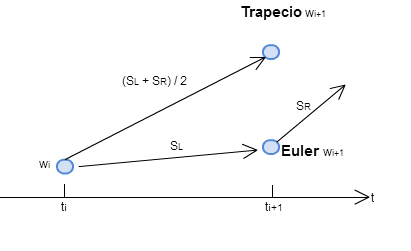
\includegraphics[width=10cm]{./Images/trapecio-vs-euler.png}
			\caption{Esquema visual del método del trapecio explícito.} 
			\label{fig:trapecio-vs-euler}
		\end{figure}

	\subsection{Método del trapecio implícito}


		Aktison

%-----------------------------------------------------------------------------------------------------
%	SECCIÓN X: ERROR
%-----------------------------------------------------------------------------------------------------


\section{Estudio del error. Convergencia}

	\subsection{Método del trapecio explícito}
	
	\subsection{Método del trapecio implícito}


%-----------------------------------------------------------------------------------------------------
%	SECCIÓN X: ESTABILIDAD
%-----------------------------------------------------------------------------------------------------

\section{Estabilidad}

%-----------------------------------------------------------------------------------------------------
%	SECCIÓN X: CONCLUSIÓN
%-----------------------------------------------------------------------------------------------------

\section{Conclusión}


%-----------------------------------------------------------------------------------------------------
%	SECCIÓN X: REFERENCIAS
%-----------------------------------------------------------------------------------------------------

\printbibliography


\end{document}
